\def\systemfont{\footnotesize}

\def\vsep{0.5}
\def\hsep{0.65}
\def\edgeopacity{0.5}

\newcommand{\neuron}[3][uiogreen]{
    \node[circle, draw=black, fill=#1, minimum size=0.3cm] (#2) at #3 {};
}

\begin{frame}{Forklarbarhetsproblemet med kunstig intelligens}
    \begin{tikzpicture}
        \node[] at (-7, -3.25) {};
        \node[] at (7, 3.25) {};

        \only<1>{
            \mriside{-4.5}{-1.4175}{1.5cm}{data/mri_sagittal.png}
            \cnnarrow{(input.east)}{($ (input.center) + (3, 0) $)}{black}
            \cnn{-2.7}{-1.4175}{0.1}{0.15}{uiogreen}{1}
            \node[anchor=west, align=left, font=\normalfont\linespread{0.9}\selectfont] (output1) at ($ (3.55, -1.4175) + (0, 0.5) $) {Pasient};
            \cnnarrow{($ (output1.west) - (1, 0.5) $)}{($ (output1.west) + (0.1, 0) $)}{black}
            \node[anchor=west, align=left, font=\normalfont\linespread{0.9}\selectfont] (output2) at ($ (3.55, -1.4175) - (0, 0.5) $) {Frisk\\kontroll};
            \cnnarrow{($ (output2.west) - (1, -0.5) $)}{($ (output2.west) + (0.1, 0) $)}{black}
        }

        \only<2-16>{
            \node[fill=gray!80, minimum width=4cm, minimum height=2.9cm, rounded corners=0.1cm, text=white, draw=black, font=\systemfont, anchor=south, text depth=2.4cm] (model) at (0, 0) {
                Kunstig nevralt nettverk
            };
            \only<2-4>{
                \neuron{n00}{($ (model.south) + (0, 1.25) + (-2*\hsep, -2*\vsep) $)}
                \neuron{n01}{($ (n00) + (0, \vsep) $)}
                \neuron{n02}{($ (n00) + (0, 2*\vsep) $)}
                \neuron{n03}{($ (n00) + (0, 3*\vsep) $)}
                \neuron{n04}{($ (n00) + (0, 4*\vsep) $)}
            }
            \only<5-14>{
                \neuron[uiogreen!60]{n00}{($ (model.south) + (0, 1.25) + (-2*\hsep, -2*\vsep) $)}
                \neuron[uiogreen!30]{n01}{($ (n00) + (0, \vsep) $)}
                \neuron[uiogreen!50!black]{n02}{($ (n00) + (0, 2*\vsep) $)}
                \neuron[uiogreen!70]{n03}{($ (n00) + (0, 3*\vsep) $)}
                \neuron[uiogreen!35!black]{n04}{($ (n00) + (0, 4*\vsep) $)}
            }
            \only<15->{
                \neuron[red!25!black]{n00}{($ (model.south) + (0, 1.25) + (-2*\hsep, -2*\vsep) $)}
                \neuron[red!90!black]{n01}{($ (n00) + (0, \vsep) $)}
                \neuron[yellow!15!red]{n02}{($ (n00) + (0, 2*\vsep) $)}
                \neuron[red!99!black]{n03}{($ (n00) + (0, 3*\vsep) $)}
                \neuron[red!10!black]{n04}{($ (n00) + (0, 4*\vsep) $)}
            }

            \only<2-5>{
                \neuron{n10}{($ (n00) + (\hsep, 0.5*\vsep) $)}
                \neuron{n11}{($ (n00) + (\hsep, 1.5*\vsep) $)}
                \neuron{n12}{($ (n00) + (\hsep, 2.5*\vsep) $)}
                \neuron{n13}{($ (n00) + (\hsep, 3.5*\vsep) $)}
            }
            \only<6-13>{
                \neuron[uiogreen!80!black]{n10}{($ (n00) + (\hsep, 0.5*\vsep) $)}
                \neuron[uiogreen!20]{n11}{($ (n00) + (\hsep, 1.5*\vsep) $)}
                \neuron[uiogreen!50]{n12}{($ (n00) + (\hsep, 2.5*\vsep) $)}
                \neuron[uiogreen!90]{n13}{($ (n00) + (\hsep, 3.5*\vsep) $)}
            }
            \only<14->{
                \neuron[red!55!black]{n10}{($ (n00) + (\hsep, 0.5*\vsep) $)}
                \neuron[yellow!20!red]{n11}{($ (n00) + (\hsep, 1.5*\vsep) $)}
                \neuron[yellow!90!red]{n12}{($ (n00) + (\hsep, 2.5*\vsep) $)}
                \neuron[red!7!black]{n13}{($ (n00) + (\hsep, 3.5*\vsep) $)}
            }

            \only<2-6>{
                \neuron{n20}{($ (n00) + (2*\hsep, \vsep) $)}
                \neuron{n21}{($ (n00) + (2*\hsep, 2*\vsep) $)}
                \neuron{n22}{($ (n00) + (2*\hsep, 3*\vsep) $)}
            }
            \only<7-12>{
                \neuron[uiogreen!80!black]{n20}{($ (n00) + (2*\hsep, \vsep) $)}
                \neuron[uiogreen!55!black]{n21}{($ (n00) + (2*\hsep, 2*\vsep) $)}
                \neuron[uiogreen!45]{n22}{($ (n00) + (2*\hsep, 3*\vsep) $)}
            }
            \only<13->{
                \neuron[red!90!black]{n20}{($ (n00) + (2*\hsep, \vsep) $)}
                \neuron[red!30!black]{n21}{($ (n00) + (2*\hsep, 2*\vsep) $)}
                \neuron[yellow!70!red]{n22}{($ (n00) + (2*\hsep, 3*\vsep) $)}
            }

            \only<2-7>{
                \neuron{n30}{($ (n00) + (3*\hsep, 1.5*\vsep) $)}
                \neuron{n31}{($ (n00) + (3*\hsep, 2.5*\vsep) $)}
            }
            \only<8-11>{
                \neuron[uiogreen!70]{n30}{($ (n00) + (3*\hsep, 1.5*\vsep) $)}
                \neuron[uiogreen!33]{n31}{($ (n00) + (3*\hsep, 2.5*\vsep) $)}
            }
            \only<12->{
                \neuron[yellow!40!red]{n30}{($ (n00) + (3*\hsep, 1.5*\vsep) $)}
                \neuron[red!65!black]{n31}{($ (n00) + (3*\hsep, 2.5*\vsep) $)}
            }

            \only<2-8>{
                \neuron{n40}{($ (n00) + (4*\hsep, 2*\vsep) $)}
            }
            \only<9-10>{
                \neuron[uiogreen!20]{n40}{($ (n00) + (4*\hsep, 2*\vsep) $)}
            }
            \only<11->{
                \neuron[red]{n40}{($ (n00) + (4*\hsep, 2*\vsep) $)}
            }

            \foreach \j in {0,...,4} {
                \draw[draw=black, alt=<5>{draw=yellow}{}, alt=<16>{draw=red}{}, opacity=\edgeopacity] ($ (model.west) - (0, 0.2175) $) -- (n0\j);
            }

            \foreach \j in {0,...,4} {
                \foreach \k in {0,...,3} {
                    \draw[draw=black, alt=<6>{draw=yellow}{}, alt=<15>{draw=red}{}, opacity=\edgeopacity] (n0\j) -- (n1\k);
                }
            }
            \foreach \j in {0,...,3} {
                \foreach \k in {0,...,2} {
                    \draw[draw=black, alt=<7>{draw=yellow}{}, alt=<14>{draw=red}{}, opacity=\edgeopacity] (n1\j) -- (n2\k);
                }
            }
            \foreach \j in {0,...,2} {
                \foreach \k in {0,...,1} {
                    \draw[draw=black, alt=<8>{draw=yellow}{}, alt=<13>{draw=red}{}, opacity=\edgeopacity] (n2\j) -- (n3\k);
                }
            }
            \draw[draw=black, alt=<9>{draw=yellow}{}, alt=<12>{draw=red}{}, opacity=\edgeopacity] (n30) -- (n40);
            \draw[draw=black, alt=<9>{draw=yellow}{}, alt=<12>{draw=red}{}, opacity=\edgeopacity] (n31) -- (n40);
            \draw[draw=black, alt=<10>{draw=yellow}{}, alt=<11>{draw=red}{}, opacity=\edgeopacity] (n40) -- ($ (model.south east) + (0, 1.25) $);
        }
        \only<2-3>{
            \node[circle, draw=black, fill=uiogreen, minimum size=0.5cm] (neuron) at (0, -1.7) {};

            \node[anchor=east, font=\scriptsize] (x1) at ($ (neuron) - (0.75, -0.5) $) {$\text{input}_1$};
            \node[anchor=east, font=\scriptsize] (x2) at ($ (neuron) - (0.75, 0) $) {$\text{input}_2$};
            \node[anchor=east, font=\scriptsize] (x3) at ($ (neuron) - (0.75, 0.5) $) {$\text{input}_3$};

            \node[anchor=west, font=\scriptsize] (y) at ($ (neuron) + (0.75, 0) $) {$\text{output}$};

            \draw[-stealth] (x1) -- (neuron);
            \draw[-stealth] (x2) -- (neuron);
            \draw[-stealth] (x3) -- (neuron);
            \draw[-stealth] (neuron) -- (y);

            \node[font=\small] at ($ (neuron) + (0, 1) $) {
                Kunstig nevron
            };
        }
        \only<3>{
            \node[font=\small] at (0, -2.75) {
                $\text{output}=\text{max}(0, b+\text{input}_1*w_1+\text{input}_2*w_2+\text{input}_3*w_3)$
            };
        }
        \only<4-16>{
            \node[anchor=east, inner sep=0pt, draw=black] (input) at (-3, 1.25) {
                \only<4-15>{%
                    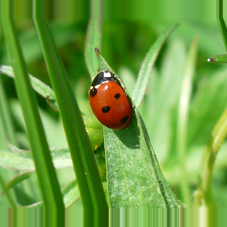
\includegraphics[width=2.5cm]{data/ladybug.png}
                }%
                \only<16>{%
                    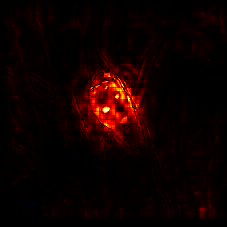
\includegraphics[width=2.5cm]{data/ladybug_explanation.png}
                }%
            };
            \draw[alt=<16>{draw=red, stealth-}{draw=black, -stealth}] (input) -- ($ (model.west) - (0, 0.2175) $);
        }
        \only<10-16>{
            \node[anchor=west, alt=<12->{text=red}{text=black}] (output) at (3, 1.25) {$\text{marihøne}$};
            \draw[
                alt=<10>{draw=yellow, -stealth},
                alt=<11>{draw=red, stealth-}
            ] ($ (model.south east) + (0, 1.25) $) -- (output);
        }
    \end{tikzpicture}
\end{frame}


\definecolor{cases-default}{HTML}{EB5353}
\definecolor{controls-default}{HTML}{0079FF}
\definecolor{healthy-default}{HTML}{36AE7C}
\definecolor{baseline}{HTML}{FAEAB1}
\definecolor{preds}{HTML}{E5BA73}
\definecolor{maps}{HTML}{C58940}

\definecolor{color0}{rgb}{0.62, 0.004, 0.259}
\definecolor{color1}{rgb}{0.755, 0.154, 0.291}
\definecolor{color2}{rgb}{0.866, 0.29, 0.298}
\definecolor{color3}{rgb}{0.943, 0.406, 0.268}
\definecolor{color4}{rgb}{0.975, 0.557, 0.323}
\definecolor{color5}{rgb}{0.993, 0.709, 0.403}
\definecolor{color6}{rgb}{0.995, 0.832, 0.506}
\definecolor{color7}{rgb}{0.998, 0.926, 0.625}
\definecolor{color8}{rgb}{0.998, 0.999, 0.746}
\definecolor{color9}{rgb}{0.937, 0.975, 0.65}
\definecolor{color10}{rgb}{0.838, 0.935, 0.609}
\definecolor{color11}{rgb}{0.693, 0.876, 0.639}
\definecolor{color12}{rgb}{0.527, 0.811, 0.645}
\definecolor{color13}{rgb}{0.368, 0.725, 0.662}
\definecolor{color14}{rgb}{0.24, 0.582, 0.721}
\definecolor{color15}{rgb}{0.267, 0.441, 0.698}
\definecolor{color16}{rgb}{0.369, 0.31, 0.635}

\newcommand{\mriwidth}{2.2cm}
\newcommand{\gap}{0.00cm}

\newcommand{\prognostic}{
    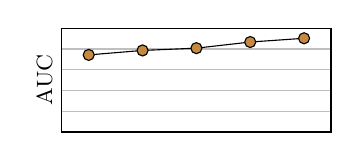
\begin{tikzpicture}
        \begin{axis}[
            height=2.9cm,
            width=5cm,
            xmajorticks=false,
            xmin=0.5,
            xmax=5.5,
            ymin=0,
            ymax=1,
            ylabel=\footnotesize{AUC},
            ymajorticks=false,
            ymajorgrids=true
        ]

            \addplot[mark=*, draw=black, mark options={fill=maps}] coordinates {
                (1, 0.743)
                (2, 0.786)
                (3, 0.808)
                (4, 0.867)
                (5, 0.903)
            };

        \end{axis}
    \end{tikzpicture}
}

\newsavebox{\prognosticheatmaps}
\sbox{\prognosticheatmaps}{
    \prognostic
}

\newcommand{\mciconcept}[1]{
    \begin{tikzpicture}
        \begin{axis}[
            height=0.47\textwidth,
            width=0.8\textwidth,
            xlabel={Tid},
            ylabel={Kognitiv funksjon},
            ticks=none,
            axis x line=bottom,
            axis y line=left,
            y axis line style={-|},
            xmin=0,
            xmax=1.4,
            ymin=0,
            ymax=1,
            clip=false
        ]
            \addplot[draw=healthy-default, smooth, line width=4pt, opacity=0.5] coordinates {
                (0, 0.9)
                (0.25, 0.87)
                (0.5, 0.77)
                (0.6, 0.72)
                (0.8, 0.63)
                (0.9, 0.72)
                (1.4, 0.67)
            };
            \addplot[draw=controls-default, smooth, line width=4pt, opacity=0.5] coordinates {
                (0, 0.9)
                (0.25, 0.87)
                (0.5, 0.77)
                (0.6, 0.72)
                (0.8, 0.63)
                (0.9, 0.61)
                (1.4, 0.54)
            };
            \addplot[draw=cases-default, smooth, line width=4pt, opacity=0.5] coordinates {
                (0, 0.9)
                (0.25, 0.87)
                (0.5, 0.77)
                (0.6, 0.72)
                (0.8, 0.625)
                (1.1, 0.48)
                (1.4, 0.3)
            };
            \addplot[dashed] coordinates {
                (0, 0.65)
                (1.4, 0.65)
            };
            \addplot[dashed] coordinates {
                (0, 0.4)
                (1.4, 0.4)
            };
            \node[anchor=south west] at (axis cs: 0, 0.64) {\footnotesize{Normal}};
            \node[anchor=north west] at (axis cs: 0, 0.66) {\footnotesize{Mild kognitiv svikt}};
            \node[anchor=north west] at (axis cs: 0, 0.41) {\footnotesize{Demens}};

            \node[anchor=west] at (axis cs: 1.4, 0.67) {\textcolor{healthy-default}{\footnotesize{Forbigående (n=80)}}};
            \node[anchor=west] at (axis cs: 1.4, 0.53) {\textcolor{controls-default}{\footnotesize{Stabile (n=754)}}};
            \node[anchor=west] at (axis cs: 1.4, 0.3) {\textcolor{cases-default}{\footnotesize{Progressive (n=354)}}};


            \ifnum#1>0
                \draw[-stealth, red, thick] (axis cs: 0.8, 0.8) -- (axis cs: 0.8, 0.67);
                \node[anchor=south] at (axis cs: 0.8, 0.8) {\textcolor{red}{\footnotesize{t}}};
            \fi

            \ifnum#1>1
                \draw[densely dotted] (axis cs: 0.9, 0.8) -- (axis cs: 0.9, 0.3);
                \draw[densely dotted] (axis cs: 1, 0.8) -- (axis cs: 1, 0.3);
                \draw[densely dotted] (axis cs: 1.1, 0.8) -- (axis cs: 1.1, 0.3);
                \draw[densely dotted] (axis cs: 1.2, 0.8) -- (axis cs: 1.2, 0.3);
                \draw[densely dotted] (axis cs: 1.3, 0.8) -- (axis cs: 1.3, 0.3);
                \node[anchor=south] at (axis cs: 0.9, 0.8) {\footnotesize{t+1}};
                \node[anchor=south] at (axis cs: 1, 0.8) {\footnotesize{t+2}};
                \node[anchor=south] at (axis cs: 1.1, 0.8) {\footnotesize{t+3}};
                \node[anchor=south] at (axis cs: 1.2, 0.8) {\footnotesize{t+4}};
                \node[anchor=south] at (axis cs: 1.3, 0.8) {\footnotesize{t+5}};
            \fi

            \ifnum#1=3
                \node[anchor=west] at (axis cs: 0.731, 0.155) {
                    \usebox{\prognosticheatmaps}
                };
			    \node[anchor=west] at (axis cs: 1.24, 0.21) {\footnotesize{0.90}};
            \fi

        \end{axis}
    \end{tikzpicture}
}

\newsavebox{\mcitrajectories}
\sbox{\mcitrajectories}{
    \mciconcept{0}
}
\newsavebox{\mcitimepoint}
\sbox{\mcitimepoint}{
    \mciconcept{1}
}
\newsavebox{\mcifuture}
\sbox{\mcifuture}{
    \mciconcept{2}
}
\newsavebox{\mciheatmaps}
\sbox{\mciheatmaps}{
    \mciconcept{3}
}
\newcommand{\correlationplot}[4]{
    \begin{tikzpicture}
        \begin{axis}[
            height=1.71 * \mriwidth,
            width=1.71 * \mriwidth,
            xmajorticks=false,
            ylabel=#3,
            ytick={0, 2, 4, 6, 8},
            yticklabels=#2,
            xmin=-1,
            xmax=17,
            ymin=0,
            ymax=9,
            every tick label/.append style={font=\tiny},
            ytick pos=left,
            scatter/classes={
                ADNI_EF={color0, draw=black},
                ADNI_MEM={color1, draw=black},
                CDCARE={color2, draw=black},
                CDCOMMUN={color3, draw=black},
                CDGLOBAL={color4, draw=black},
                CDHOME={color5, draw=black},
                CDJUDGE={color6, draw=black},
                CDMEMORY={color7, draw=black},
                CDORIENT={color8, draw=black},
                FAQTOTAL={color9, draw=black},
                GDTOTAL={color10, draw=black},
                MMSCORE={color11, draw=black},
                NPISCORE={color12, draw=black},
                PHC_EXF={color13, draw=black},
                PHC_LAN={color14, draw=black},
                PHC_MEM={color15, draw=black},
                PHC_VSP={color16, draw=black}
            },
            y label style={at={(-0.1,0.5)}},
            ymajorgrids=true,
            ytick style={draw=none},
            clip=false,
            grid style={draw=gray!20},
            axis line style={draw=gray!70}
        ]
            \addplot[
                only marks,
                scatter,
                scatter src=explicit symbolic
            ] table [
                col sep=comma,
                x=index,
                y=component_#1,
                meta=symptom
            ] {data/correlations.csv};
            \addplot[dashed,red, thick] coordinates {
                (-1, 2.76)
                (17, 2.76)
            };
            #4
        \end{axis}
    \end{tikzpicture}
}

\newsavebox{\firstcorrelations}
\sbox{\firstcorrelations}{%
    \correlationplot{0}{{0, 2, 4, 6, 8}}{\scriptsize{$-log_{10}(p)$}}{
        \node[] at (axis cs: 14, 6.19) {\tiny{PHC\_LAN}};
    }
}
\newsavebox{\secondcorrelations}
\sbox{\secondcorrelations}{%
    \correlationplot{1}{{,,}}{{}}{
        \node[] at (axis cs: 9, 3.74) {\tiny{FAQTOTAL}};
    }
}
\newsavebox{\thirdcorrelations}
\sbox{\thirdcorrelations}{%
    \correlationplot{2}{{,,}}{{}}{
        \node[] at (axis cs: 0, 6.44) {\tiny{ADNI\_EF}};
        \node[] at (axis cs: 13, 7.95) {\tiny{PHC\_EXF}};
    }
}
\newsavebox{\fourthcorrelations}
\sbox{\fourthcorrelations}{%
    \correlationplot{3}{{,,}}{{}}{
        \node[] at (axis cs: 0, 9.02) {\tiny{ADNI\_EF}};
        \node[] at (axis cs: 13, 8.75) {\tiny{PHC\_EXF}};
        \node[] at (axis cs: 14, 5.84) {\tiny{PHC\_LAN}};
        \node[] at (axis cs: 6, 5.18) {\tiny{CDJUDGE}};
        \node[] at (axis cs: 11, 3.99) {\tiny{MMSCORE}};
    }
}

\newcommand{\cognitiveplot}[1]{
    \hspace{-0.6cm}
    \begin{tikzpicture}
        \node[] (first) at (0, 0) {
            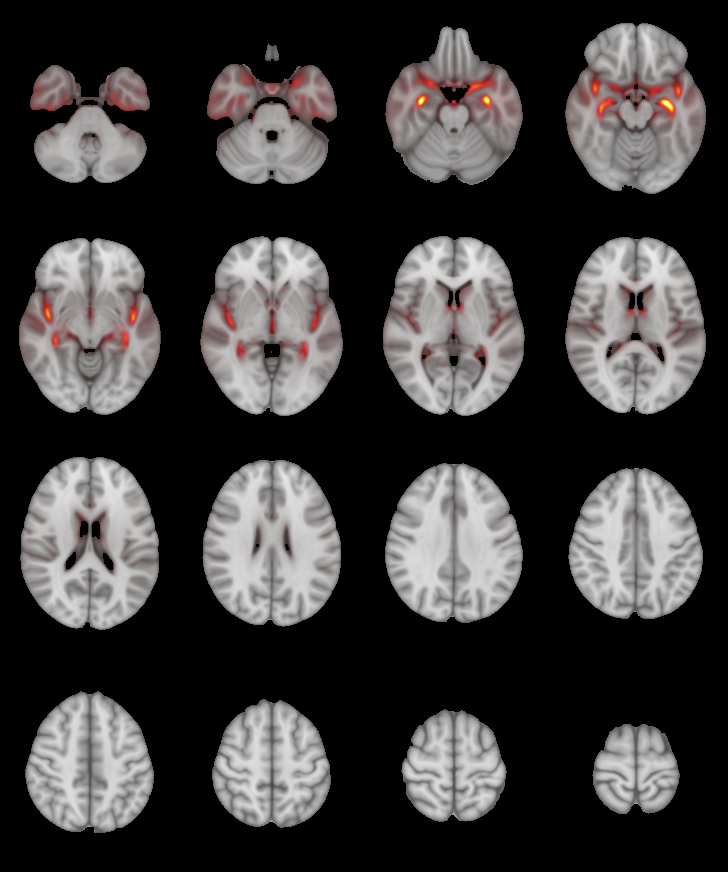
\includegraphics[
                width=\mriwidth,
                clip=true,
                trim = 192mm 232mm 0mm 0mm
            ]{data/components/component_0.png}
        };

        \node[anchor=west] (second) at ($ (first.east) + (\gap, 0) $) {
            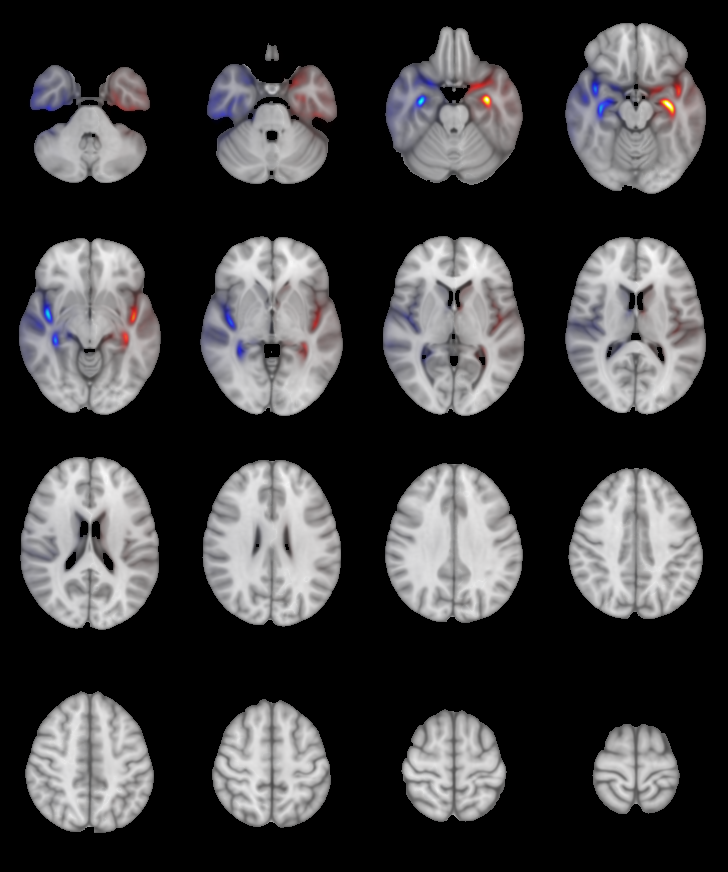
\includegraphics[
                width=\mriwidth,
                clip=true,
                trim = 192mm 232mm 0mm 0mm
            ]{data/components/component_1.png}
        };

        \node[anchor=west] (third) at ($ (second.east) + (\gap, 0) $) {
            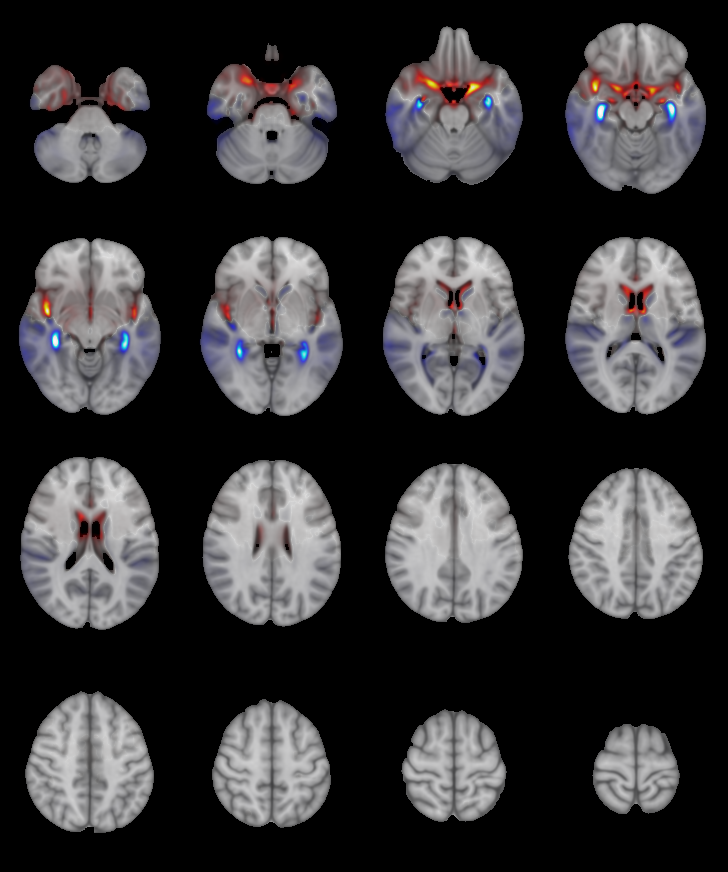
\includegraphics[
                width=\mriwidth,
                clip=true,
                trim = 192mm 232mm 0mm 0mm
            ]{data/components/component_2.png}
        };

        \node[anchor=west] (fourth) at ($ (third.east) + (\gap, 0) $) {
            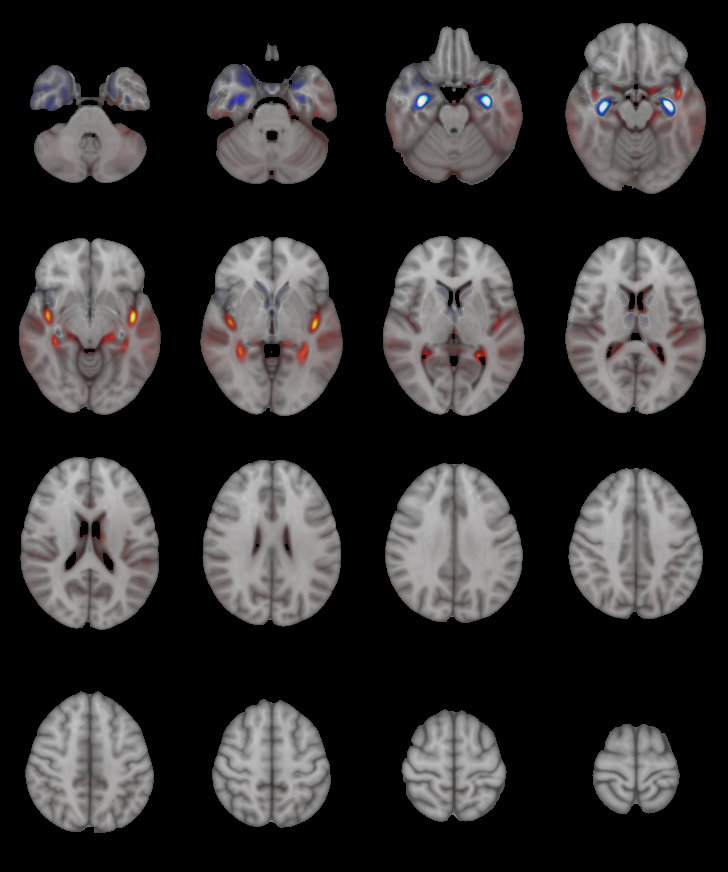
\includegraphics[
                width=\mriwidth,
                clip=true,
                trim = 192mm 232mm 0mm 0mm
            ]{data/components/component_3.png}
        };

        \ifnum#1=1
            \node[anchor=north west] (first-correlation) at ($ (first.south west) + (-0.86, 0.1) $) {
                \usebox{\firstcorrelations}
            };
            \node[anchor=north west] (second-correlation) at ($ (first-correlation.north east) - (0.76, 0) $) {
                \usebox{\secondcorrelations}
            };
            \node[anchor=north west] (third-correlation) at ($ (second-correlation.north east) - (0.71, 0) $) {
                \usebox{\thirdcorrelations}
            };
            \node[anchor=north west] (fourth-correlation) at ($ (third-correlation.north east) - (0.74, -0.21) $) {
                \usebox{\fourthcorrelations}
            };
        \fi

    \end{tikzpicture}
    \hspace{-0.6cm}
}

\newsavebox{\cognitiveheatmaps}
\sbox{\cognitiveheatmaps}{
    \cognitiveplot{0}
}

\newsavebox{\cognitivecorrelations}
\sbox{\cognitivecorrelations}{
    \cognitiveplot{1}
}

\begin{frame}{Forklarbar kunstig intelligens og demens}
    \begin{tikzpicture}
        \node[] at (-7, -3.25) {};
        \node[] at (7, 3.25) {};

        \node[anchor=south, font=\tiny, text width=10.5cm, align=flush center] at (0, -3.4) {
            Esten H. Leonardsen et al., Constructing personalized characterizations of structural brain aberrations in patients with dementia using explainable artificial intelligence. \textit{npj Digital Medicine} (2024)
        };

        \only<1>{
            \mriside{-4.5}{-0.2175}{1.5cm}{data/mri_sagittal.png}
            \cnnarrow{(input.east)}{($ (input.center) + (3, 0) $)}{black}
            \cnn{-2.7}{-0.2175}{0.1}{0.15}{uiogreen}{1}
            \node[anchor=west, align=left, font=\normalfont\linespread{0.9}\selectfont] (output1) at ($ (3.55, -0.2175) + (0, 0.5) $) {Demens-\\pasient};
            \cnnarrow{($ (output1.west) - (1, 0.5) $)}{($ (output1.west) + (0.1, 0) $)}{black}
            \node[anchor=west, align=left, font=\normalfont\linespread{0.9}\selectfont] (output2) at ($ (3.55, -0.2175) - (0, 0.5) $) {Frisk\\kontroll};
            \cnnarrow{($ (output2.west) - (1, -0.5) $)}{($ (output2.west) + (0.1, 0) $)}{black}
        }
        \only<2>{
            \mriside{-4.5}{-0.2175}{1.5cm}{data/combined_sagittal.png}
            \lrparrow{($ (input.center) + (3, 0) $)}{(input.east)}{black}
            \lrp{-2.7}{-0.2175}{0.1}{0.15}
            \node[anchor=west, align=left, font=\normalfont\linespread{0.9}\selectfont] (output1) at ($ (3.55, -0.2175) + (0, 0.5) $) {Demens-\\pasient};
            \lrparrow{($ (output1.west) + (0.1, 0) $)}{($ (output1.west) - (1, 0.5) $)}{black}
        }

        \only<3>{
            \node[
				minimum height=0.41\textwidth,
				minimum width=0.32\textwidth,
				fill=black,
                anchor=west
			] (box1) at (-6.8, 0.3) {};
			\node[anchor=south] at (box1.south) {
				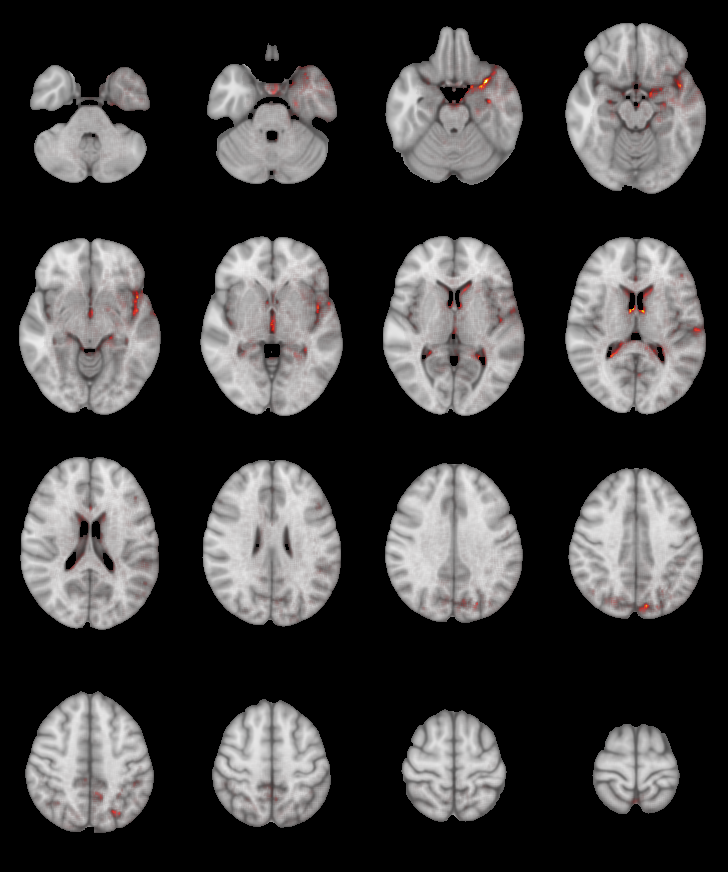
\includegraphics[width=0.31\textwidth]{data/subject1.png}
			};
			\node[anchor=north,inner sep=2pt, text=white, font=\footnotesize] at (box1.north) {Pasient 1};

			\node
				[minimum height=0.41\textwidth,
				minimum width=0.32\textwidth,
				fill=black,
				anchor=west
			] (box2) at ($ (box1.east) + (0.05,0) $) {};
			\node[anchor=south] at (box2.south) {
				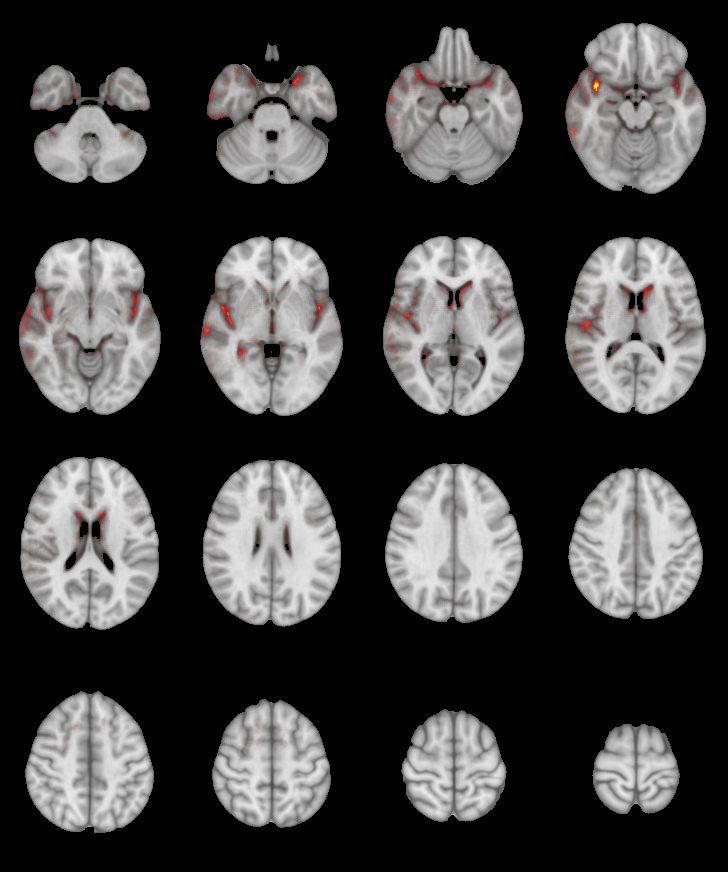
\includegraphics[width=0.31\textwidth]{data/subject2.png}
			};
			\node[anchor=north,inner sep=3pt, text=white, font=\footnotesize] at (box2.north) {Pasient 2};

			\node
				[minimum height=0.41\textwidth,
				minimum width=0.32\textwidth,
				fill=black,
				anchor=west
			] (box3) at ($ (box2.east) + (0.05,0) $) {};
			\node[anchor=south] at (box3.south) {
				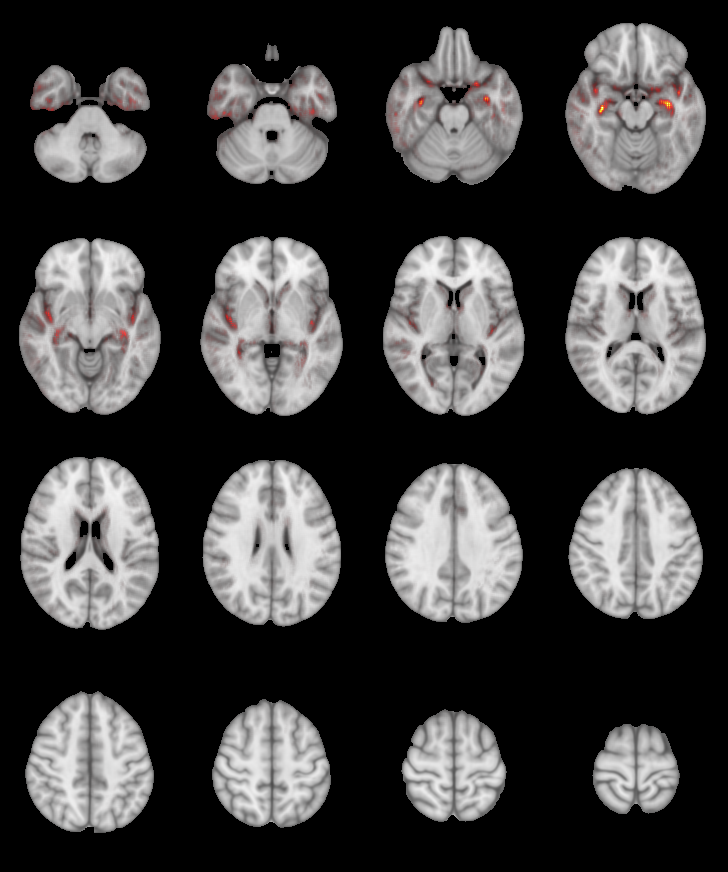
\includegraphics[width=0.31\textwidth]{data/subject3.png}
			};
			\node[anchor=north,inner sep=3pt, text=white, font=\footnotesize] at (box3.north) {Pasient 3};
        }
        \only<4-5>{
            \node[label={[text depth=0, inner sep=2pt]above:Forklarbar KI}] at (-2.5, 0.25) {
				
\includegraphics[width=0.31\textwidth]{data/dementia.png}
			};
        }
        \only<5>{
			\node[label={[text depth=0, inner sep=2pt]above:Mennesker}] at (2.5, 0.25) {
				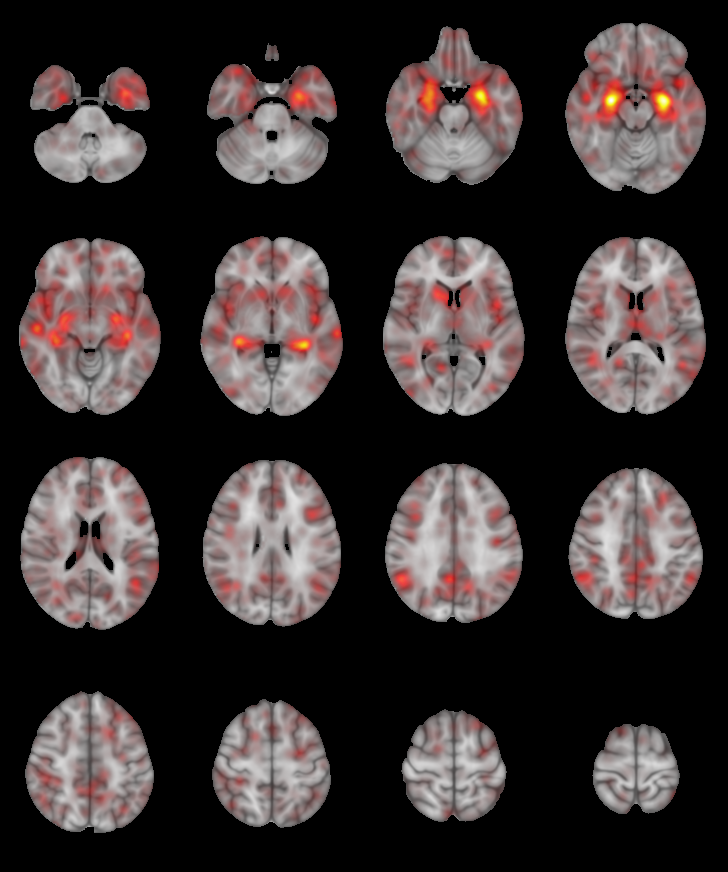
\includegraphics[width=0.31\textwidth]{data/ALE.png}
			};
        }

        \only<6>{
            \node[] at (0, 0.35) {
                \usebox{\mcitrajectories}
            };
        }

        \only<7>{
            \node[] at (0, 0.35) {
                \usebox{\mcitimepoint}
            };
        }
        \only<8>{
            \node[] at (0, 0.35) {
                \usebox{\mcifuture}
            };
        }
        \only<9>{
            \node[] at (0, 0.35) {
                \usebox{\mciheatmaps}
            };
        }

        \visible<10>{
            \node[inner sep=0pt, outer sep=0pt, anchor=north east] at (4.6, 3) {
                \usebox{\cognitiveheatmaps}
            };
        }
        \visible<11>{
            \node[inner sep=0pt, outer sep=0pt, anchor=north east] at (5, 3) {
                \usebox{\cognitivecorrelations}
            };
        }
    \end{tikzpicture}
\end{frame}
